here we compare the volumetric plane-tree to the ot, the other methods are designed for mesh compression and since the ot is one of the most common representations used for 3d reconstruction we compare with it. we also have an implementation of ilqt extended to 3d called the ilot (interpolating leaf oct-tree) we compare with. Results show that for low bit-rates the ilot outperforms the ot. However as higher quality is required, OT outperforms this. The plane-tree which was the original envisionment of iqlt for 3D data is shown to improve upon the OT and ILOT at both low and high bit-rates. \\

\begin{figure*}[t]
\centering
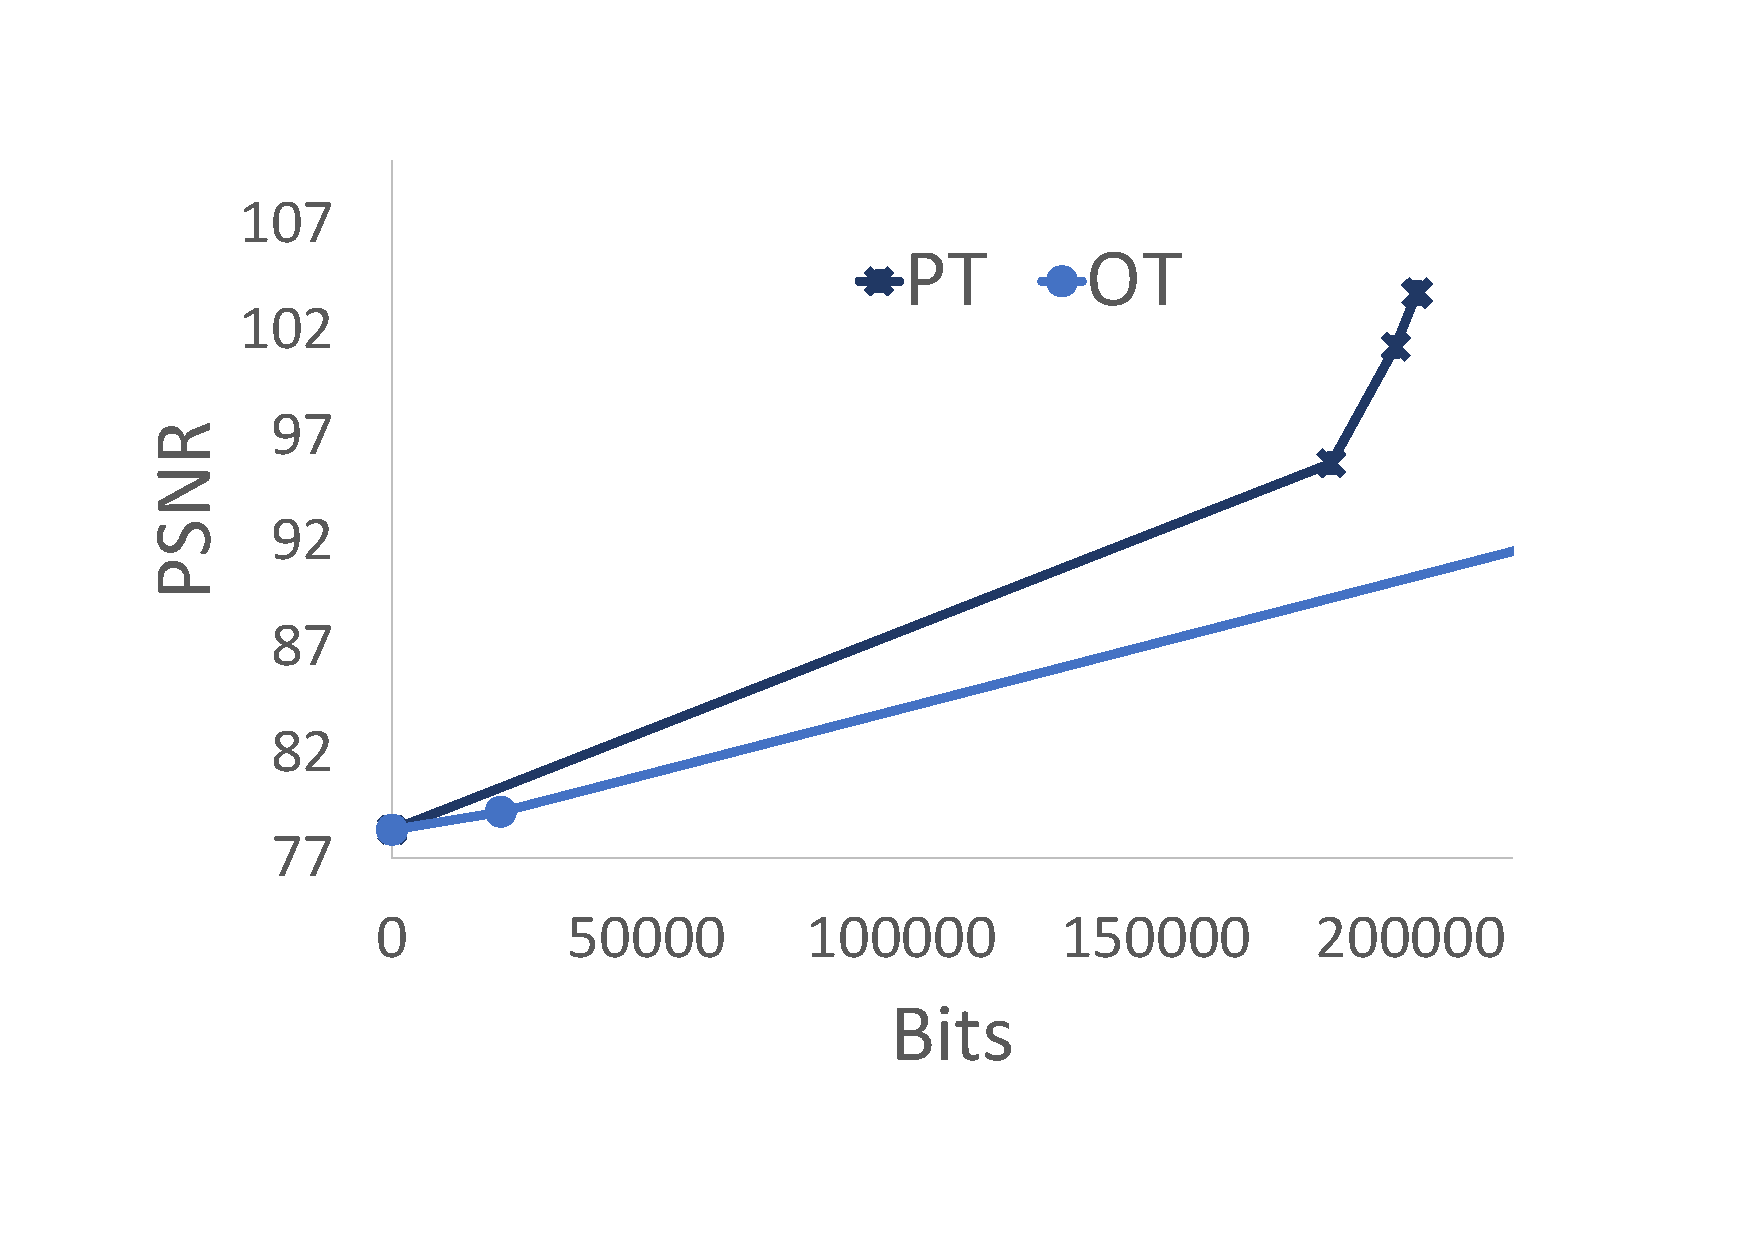
\includegraphics[width=6.0in]{images/results/compression/psnr1}
\caption{PSNR vs Bitrate comparing the ILOT, OT and PT compression methods.}
\label{fig:PSNR1}
\end{figure*}

By reducing the size of 3D reconstructions processing speed and storage will be advanced. This is advantageous in 3D reconstruction as we may want to transmit reconstructions over a network (from a robot to a base station for example). By using an advanced compression scheme we can transmit this data faster. 